\documentclass[aspectratio=169]{beamer}
%\documentclass{easytikz}


\usepackage{default}
\usepackage{tikz}
\usetikzlibrary{positioning,automata,calc}
\usepackage{multicol}


%\usepackage{timing}

\usepackage[utf8]{inputenc}
\usepackage[T1]{fontenc}
\usepackage{minibox}
\usepackage{setspace}



\usetikzlibrary{shapes.geometric, arrows}
\usetikzlibrary{positioning}


\title{Authentifizierung -- Client Certificate}
\subtitle{Das Ende der Passwörter}
\author{Stefan Helmert}
\institute{entroserv.de}
\date{02/2020}

\logo{\Large\texttt{\minibox{entroserv\vspace{-.27cm}\\\hspace{0.63cm} course}}}

\tikzset{
  nd/.style={rectangle, rounded corners, minimum width=3cm, minimum height=1cm,text centered, draw=black},
  off/.style={rectangle, rounded corners, minimum width=3cm, minimum height=1cm,text centered, draw=black, fill=red},
  se/.style={rectangle, rounded corners, minimum width=3cm, minimum height=1cm,text centered, draw=black, fill=red!30},
  sed/.style={rectangle, rounded corners, minimum width=3cm, minimum height=1cm,text centered, draw=black, fill=black!30},
  io/.style={trapezium, trapezium left angle=70, trapezium right angle=110, minimum width=3cm, minimum height=1cm, text centered, draw=black, fill=blue!30},
  op/.style={rectangle, minimum width=3cm, minimum height=1cm, text centered, draw=black, fill=orange!30},
  cn/.style={diamond, minimum width=3cm, minimum height=1cm, text centered, draw=black, fill=green!30},
  sc/.style={circle, minimum width=2cm, minimum height=1cm, text centered, draw=black, fill=blue!30},
  node distance=7mm
}

\begin{document}
	
\frame{\titlepage}


\begin{frame}
\tableofcontents
\end{frame}


\section{Ausgangssituation}
\subsection{Geteiltes Geheimnis}
\begin{frame}[fragile]{\insertsection}{\insertsubsection}

\textbf{Authtoken}

\begin{multicols}{2}
	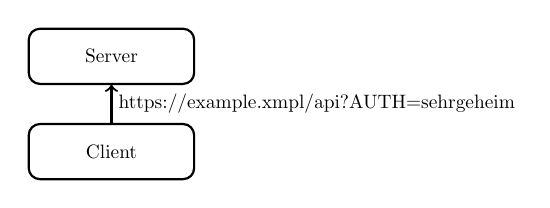
\begin{tikzpicture}[thick,scale=0.7, every node/.style={transform shape}]
	\node[nd] (server) {Server};
	\node[nd, below=of server] (client) {Client};
	\draw[->] (client) -- node[right] {https://example.xmpl/api?AUTH=sehrgeheim} (server);
	\end{tikzpicture}
	\begin{itemize}
		\item jeder Client im Server registriert
		\item Server kennt Geheimnis
		\item Client kennt Geheimnis
		\item Übertragungsweg erfährt Geheimnis
	\end{itemize}
\end{multicols}
\end{frame}


\begin{frame}[fragile]{\insertsection}{\insertsubsection}

\textbf{Message Authentication Code}

\begin{multicols}{2}
	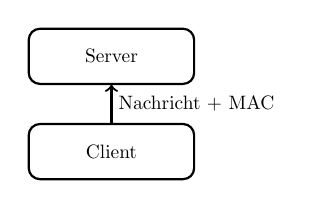
\begin{tikzpicture}[thick,scale=0.7, every node/.style={transform shape}]
	\node[nd] (server) {Server};
	\node[nd, below=of server] (client) {Client};
	\draw[->] (client) -- node[right] {Nachricht + MAC} (server);
	\end{tikzpicture}
	\begin{itemize}
		\item jeder Client im Server registriert
		\item Server kennt Geheimnis
		\item Client kennt Geheimnis
		\item Übertrag. erfährt Geheimn. nicht
	\end{itemize}
\end{multicols}
\end{frame}

\begin{frame}[fragile]{\insertsection}{\insertsubsection}

\textbf{Symmetrische Schlüssel}

\begin{multicols}{2}
	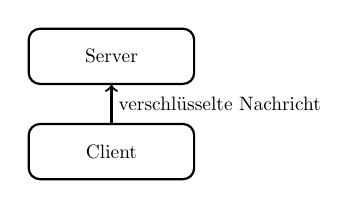
\begin{tikzpicture}[thick,scale=0.7, every node/.style={transform shape}]
	\node[nd] (server) {Server};
	\node[nd, below=of server] (client) {Client};
	\draw[->] (client) -- node[right] {verschlüsselte Nachricht} (server);
	\end{tikzpicture}
	\begin{itemize}
		\item jeder Client im Server registriert
		\item Server kennt Geheimnis
		\item Client kennt Geheimnis
		\item Übertrag. erfährt Geheimn. nicht
	\end{itemize}
\end{multicols}
\end{frame}

\subsection{Nicht geteiltes Geheimnis}

\begin{frame}[fragile]{\insertsection}{\insertsubsection}

\textbf{Asymetrische Schlüssel}

\begin{multicols}{2}
	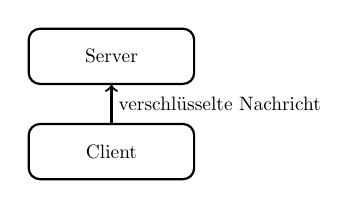
\begin{tikzpicture}[thick,scale=0.7, every node/.style={transform shape}]
	\node[nd] (server) {Server};
	\node[nd, below=of server] (client) {Client};
	\draw[->] (client) -- node[right] {verschlüsselte Nachricht} (server);
	\end{tikzpicture}
	\begin{itemize}
		\item jeder Client im Server registriert
		\item Server erfährt Geheimnis nicht
		\item Client kennt Geheimnis
		\item Übertrag. erfährt Geheimn. nicht
	\end{itemize}
\end{multicols}
\end{frame}

\section{Problem}
\subsection{Komplexität und Datenschutz}
\begin{frame}[fragile]{\insertsection}{\insertsubsection}

\textbf{Asymetrische Schlüssel}

\begin{multicols}{2}
	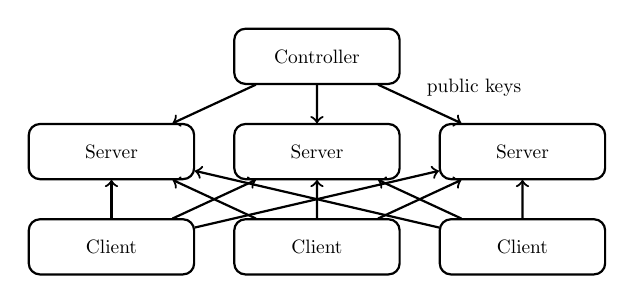
\begin{tikzpicture}[thick,scale=0.7, every node/.style={transform shape}]
	\node[nd] (server1) {Server};
	\node[nd, below=of server1] (client1) {Client};
	\node[nd, right=of server1] (server2) {Server};
	\node[nd, below=of server2] (client2) {Client};
	\node[nd, right=of server2] (server3) {Server};
	\node[nd, below=of server3] (client3) {Client};

	\draw[->] (client1) -- (server1);
	\draw[->] (client1) -- (server2);
	\draw[->] (client1) -- (server3);

	\draw[->] (client2) -- (server1);
	\draw[->] (client2) -- (server2);
	\draw[->] (client2) -- (server3);

	\draw[->] (client3) -- (server1);
	\draw[->] (client3) -- (server2);
	\draw[->] (client3) -- (server3);

	\node[nd, above=of server2] (controller) {Controller};
	\draw[->] (controller) -- (server1);
	\draw[->] (controller) -- (server2);
	\draw[->] (controller) -- node[above right] {public keys} (server3);
	\end{tikzpicture}
	\begin{itemize}
		\item jeder Client in jedem Server registriert
		\item aufwendige Schlüsselverteilung
		\item Konsistenz der Schlüssel
		\item Datenschutz -- Schlüssel als Identifikationsmerkmal
	\end{itemize}
\end{multicols}
\end{frame}

\section{Folgen}
\subsection{Inkonsistenz}
\begin{frame}[fragile]{\insertsection}{\insertsubsection}

\textbf{Asymetrische Schlüssel}

\begin{multicols}{2}
	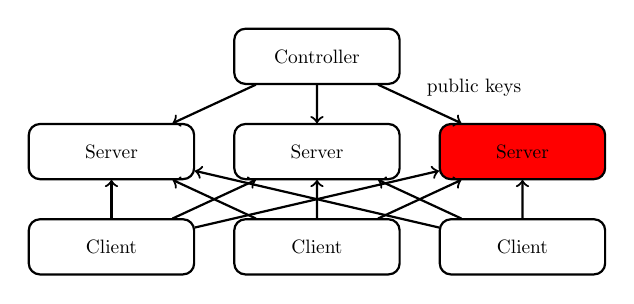
\begin{tikzpicture}[thick,scale=0.7, every node/.style={transform shape}]
	\node[nd] (server1) {Server};
	\node[nd, below=of server1] (client1) {Client};
	\node[nd, right=of server1] (server2) {Server};
	\node[nd, below=of server2] (client2) {Client};
	\node[off, right=of server2] (server3) {Server};
	\node[nd, below=of server3] (client3) {Client};
	
	\draw[->] (client1) -- (server1);
	\draw[->] (client1) -- (server2);
	\draw[->] (client1) -- (server3);
	
	\draw[->] (client2) -- (server1);
	\draw[->] (client2) -- (server2);
	\draw[->] (client2) -- (server3);
	
	\draw[->] (client3) -- (server1);
	\draw[->] (client3) -- (server2);
	\draw[->] (client3) -- (server3);
	
	\node[nd, above=of server2] (controller) {Controller};
	\draw[->] (controller) -- (server1);
	\draw[->] (controller) -- (server2);
	\draw[->] (controller) -- node[above right] {public keys} (server3);
	\end{tikzpicture}
	\begin{itemize}
		\item Server besitzt ungültigen Schlüssel
		\item Server hat neuen Schlüssel nicht
		\item abgelaufener, aber verbliebener Schlüssel verrät, welcher Client Zugriff hatte (Löschfrist DSGVO) -- Abmahnrisiko
	\end{itemize}
\end{multicols}
\end{frame}

\section{Problem}
\subsection{Komplexität und Datenschutz}
\begin{frame}[fragile]{\insertsection}{\insertsubsection}

\textbf{Asymetrische Schlüssel}

\begin{multicols}{2}
	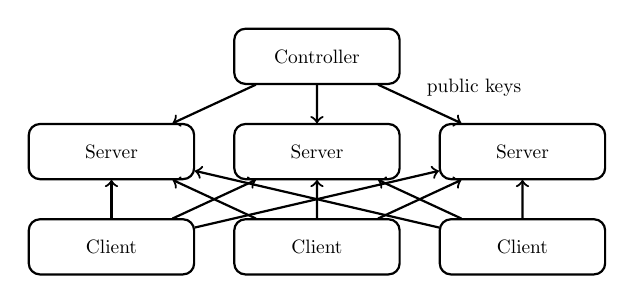
\begin{tikzpicture}[thick,scale=0.7, every node/.style={transform shape}]
	\node[nd] (server1) {Server};
	\node[nd, below=of server1] (client1) {Client};
	\node[nd, right=of server1] (server2) {Server};
	\node[nd, below=of server2] (client2) {Client};
	\node[nd, right=of server2] (server3) {Server};
	\node[nd, below=of server3] (client3) {Client};
	
	\draw[->] (client1) -- (server1);
	\draw[->] (client1) -- (server2);
	\draw[->] (client1) -- (server3);
	
	\draw[->] (client2) -- (server1);
	\draw[->] (client2) -- (server2);
	\draw[->] (client2) -- (server3);
	
	\draw[->] (client3) -- (server1);
	\draw[->] (client3) -- (server2);
	\draw[->] (client3) -- (server3);
	
	\node[nd, above=of server2] (controller) {Controller};
	\draw[->] (controller) -- (server1);
	\draw[->] (controller) -- (server2);
	\draw[->] (controller) -- node[above right] {public keys} (server3);
	\end{tikzpicture}
	\begin{itemize}
		\item jeder Client in jedem Server registriert
		\item aufwendige Schlüsselverteilung
		\item Konsistenz der Schlüssel
		\item Datenschutz -- Schlüssel als Identifikationsmerkmal
	\end{itemize}
\end{multicols}
\end{frame}

\section{Lösung}
\subsection{Public Key Infrastructure}
\begin{frame}[fragile]{\insertsection}{\insertsubsection}

\textbf{Client Certificate}

\begin{multicols}{2}
\begin{tikzpicture}[thick,scale=0.7, every node/.style={transform shape}]
\node[nd] (server1) {Server};
\node[nd, below=of server1] (client1) {Client};


\draw[->] (client1) -- node[right] {Login} (server1);


\node[nd, above=of server1] (cca) {CCA};
\draw[->] (cca) -- node[right] {Root Cert} (server1);
\draw[->] (cca) to [bend left=90] node [right] {Client Cert} (client);

\end{tikzpicture}
\begin{itemize}
	\item Server kennt nur Root Certificate
	\item Server erfährt Client Certificate nur beim Login
	\item CCA kennt Root Certificate und zugehörigen Private Key
	\item Client kennt Client Certificate und zugehörigen Private Key
\end{itemize}
\end{multicols}
\end{frame}


\begin{frame}[fragile]{\insertsection}{\insertsubsection}

\textbf{Ablauf}

\begin{multicols}{2}
	\begin{enumerate}
		\item CCA: Schlüsselpaar erzeugen
		\item CCA: Root CSR erzeugen (und pub~key anhängen)
		\item CCA: Root Cert erzeugen (CSR selfsigning)
		\item Root Cert CCA $\rightarrow$ Server
		\item Client: Schlüsselpaar erzeugen
		\item Client: CSR erzeugen (inkl. pub key)
		\item CSR Client $\rightarrow$ CCA
		\item CCA: signiert Client CSR (Ergebnis Client Cert)
		\item Client Cert CCA $\rightarrow$ Client
		\item Login-Anfrage Client $\rightarrow$ Server
		\item Challenge Server $\rightarrow$ Client
		\item Client signiert Challenge (=Response)
		\item Response + Client Cert Client~$\rightarrow$~Server
		\item Server prüft Response, Client Cert
		\item Session Server~$\leftrightarrow$~Client
	\end{enumerate}
\end{multicols}
\end{frame}



\begin{frame}[fragile]{\insertsection}{\insertsubsection}

\textbf{Intermediate Client Certificate}

\begin{multicols}{2}
	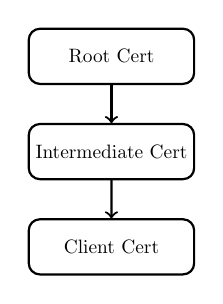
\begin{tikzpicture}[thick,scale=0.7, every node/.style={transform shape}]
	\node[nd] (root) {Root Cert};
	\node[nd, below=of root] (intermediate) {Intermediate Cert};
	\node[nd, below=of intermediate] (client) {Client Cert};
	\draw[->] (root) -- (intermediate);
	\draw[->] (intermediate) --  (client);

	
	\end{tikzpicture}
	\begin{itemize}
		\item Vererbung von Rechten
		\item keine Rechteerhöhung (Laufzeit beachten!)
		\item übergeordneter Zertifikatsinhaber kann Gültigkeit entziehen!
	\end{itemize}
\end{multicols}
\end{frame}


\end{document}




\section{Kontakt}
\begin{frame}[fragile]{\insertsection}{\insertsubsection}
\scalebox{1.2}{%
	\begin{minipage}{2\textwidth}
		\begin{description}
			\item[Folien] \url{https://github.com/TheTesla/ProgrammierTutorial}
			\item[Github] \url{https://github.com/TheTesla}
			\item[Webseite] \url{https://entroserv.de/}
			\item[Mailingliste] \url{https://www.lists.entroserv.de/listinfo/lounge}
			\item[E-Mail] \href{mailto:stefan@entroserv.de}{stefan@entroserv.de}
			\item[Telegram] @Tesla423
		\end{description}
	\end{minipage}%
}

\end{frame}